\textbf{The Nature of Attitudes Toward Artificial Intelligence in Mass Publics}

\noindent\resizebox{\textwidth}{!}{%
\begin{tabular}{c | c | c | c}
\hline
   & \textit{Ignacio Urbina} \textit{Stony Brook University} & \textit{Oleg Smirnov} \textit{Stony Brook University} &  \\
  \hline
\end{tabular}
}

\textit{March 31, 2024}

\textbf{Work in Progress. Please do not circulate.}

\textbf{Abstract}

What is the nature and structure of mass attitudes towards artificial intelligence (AI)? Despite AI's growing importance, it remains unclear whether public attitudes are consistent across different AI domains and the socio-political contexts of their use cases. This uncertainty raises a critical question: Can a 'general' attitude toward AI adequately capture citizens' perceptions toward specific AI applications, or is a model emphasizing the multidimensional nature of AI use cases and their deployment contexts more accurate? To explore the structure of AI attitudes, we conducted exploratory factor analysis on a nationally representative sample of US adults, analyzing the covariance of over fifty items across various topics and three AI applications: classification algorithms, facial recognition, and automated vehicles. Our findings indicate that AI attitudes are best described by a complex structure encompassing a general AI attitude, domain-specific opinions, and the socio-political context of AI applications. Recognizing this complexity is crucial for industry and policymakers to develop technologies and regulations that are not only effective but also equitable, aligning with the public sentiments toward AI.

\textbf{Introduction}

Artificial intelligence (AI) has seen an unprecedented adoption across many sectors of the economy and social life, from entertainment (Anantrasirichai \& Bull, 2022) and education (Baidoo-Anu \& Ansah, 2023) to healthcare (Jiang et al., 2017; Secinaro et al., 2021) and transportation (Abduljabbar et al., 2019) to law enforcement (Berk, 2021) and military technologies (Szabadföldi, 2021). The widespread adoption of AI significantly influences public opinion, which in turn impacts the technology's integration into society. This two-way dynamics is evident in various social and political domains, from individuals' likelihood to embrace the technology (Herath \& Mittal, 2022; Horowitz \& Kahn, 2021), concerns about job displacement due to AI advancements (Acemoglu \& Restrepo, 2018; Chen et al., 2022), to the readiness of the public to participate in discussions about AI regulation and policy-making (Buiten, 2019; Kieslich et al., 2022). 

Understanding public opinion on AI has emerged as a critical and timely research area for scholars and policymakers, comparable to the significance of the technology's adoption itself (Stein et al., 2024). While there exists an established body of literature on looking at public opinion and attitudes across diverse topics, the problem of artificial intelligence is novel, distinct, and unprecedented based in a multitude of factors. These may include an individual's familiarity with information technology (Horowitz et al., 2023), political ideology and views on government intervention (Cui \& van Esch, 2022), apprehensions about the unknown (Khasawneh, 2018), future-oriented thinking (Peschl \& Fundneider, 2017), susceptibility to conspiracy theories (Bruder et al., 2013), and unique psychological traits (Costa Jr \& McCrae, 1992).

Furthermore, in the context of artificial intelligence, researchers must differentiate whether they are examining a singular global attitude toward AI (Schepman \& Rodway, 2020; Stein et al., 2024) or exploring a network of interrelated attitudes, beliefs, and feelings. The dimensionality of AI attitudes—whether they are based on a single or multiple dimensions—requires thorough investigation. Thus, a principled development and testing of survey instruments to measure public opinion on AI should be the central focus of the researchers before such instruments are actually used.

In the present study, we explore the structure of AI attitudes. We ask the following questions: Are the attitudes based on a \textit{single} underlying dimension (e.g., a simple positive versus negative attitudinal space), or are they \textit{domain}-specific (e.g., personal assistants, autonomous vehicles, face recognition, and so on)? What is the role of the social and political \textit{context} surrounding those domains, and could AI attitudes, even within a single domain, differ depending on the specific application of the technology? Our substantive goal is to identify such structure based on empirical evidence and suggest a theoretical foundation for the study of AI attitudes, which is already experiencing an exponential growth of scholarly interest and practical applications by policymakers in the present and foreseeable future. Our second goal is methodological as we make suggestions with respect to measurement of AI attitudes and what survey questions would be more effective in capturing the structure of such attitudes.

Defining "artificial intelligence" (AI) presents a considerable challenge, a complexity that evolves in parallel with the technology's advancement and its societal adoption (Monett \& Lewis, 2018; Wang, 2019). John McCarthy, a foundational figure in AI, characterized it as "the science and engineering of making intelligent machines" (Rajaraman, 2014). This definition can be expanded further by the Stanford Institute for Human-Centered Artificial Intelligence, which states that intelligence entails the capacity to learn and apply techniques to address challenges and achieve goals in a dynamic environment (Auernhammer, 2020). At its essence, AI involves the design and application of intelligent machines aimed at specific outcomes. Although AI could be simplistically compared to a tool like a hammer for a carpenter, such an analogy does not adequately account for the intricate societal and political ramifications of various AI applications.

Public attitudes towards AI are shaped by a variety of factors. For instance, one’s concerns about diversity and inclusion may limit their enthusiasm about the technology if the latter is seen as a tool to perpetuate discrimination. The public perception of AI as biased or discriminatory can outweigh any proposed benefits of the technology. Normative beliefs in general—individuals' perceptions of societal norms and expectations—must play an important role in forming attitudes towards AI. Another example is a concern about privacy: individuals may be apprehensive about personal information security and, therefore, less willing to accept AI technologies. Related to that, perceptions of control and autonomy also influence attitudes toward AI: technologies perceived to diminish autonomy or make decision-making process less transparent would be met with opposition. Interestingly, the influence of conspiracy theories also cannot be overlooked (Stein et al., 2024), as they can skew public understanding and generate concerns about public surveillance or manipulation. Finally, another important determinant of public attitudes towards AI is the general trust in: (a) the entities developing artificial intelligence (e.g., OpenAI, Meta, Google), (b) the entities overseeing this development and subsequent applications (e.g., the Federal Trade Commission), and (c) the scientists and academic researchers studying the technology and communicating its risk and benefits to the public.

\textbf{Study Design and Analysis}

To identify an appropriate structure of attitudes towards artificial intelligence, we use data from Pew Research Center’s wave 99 of the American Trends Panel, a survey of 10,260 U.S. adults conducted between November 1st and 7th, 2021. The survey contains questions about the general attitudes about artificial intelligence, devoid of a particular domain, as well as the questions about specific AI applications: namely (a) facial recognition technology and surveillance, (b) the use of algorithms by social media companies to detect misinformation, and (c) the development of driverless passenger vehicles. A subset of the respondents (N = 5,153) answered questions about artificial intelligence, while the other half were asked about other technologies such as gene editing and exoskeletons.

As such our paper is not a definitive description of AI attitudes across all possible and relevant domains, nor is it an updated picture contemporary public opinion (spring of 2024 at the time of writing). Instead, our goal is to provide an illustration of a structure of AI attitudes comprised of several distinct, yet interdependent, factors, which are furthermore potentially affected by the political and social context depending on the area of application of AI. In our analysis, we are limited by the set of questions from the Pew study and by the fact that the ChatGPT technological “revolution” had yet to occur at the time of the survey.

To explore a potential structure of beliefs about artificial intelligence using a comprehensive set of survey questions related to AI from the American Trends Panel, we employ exploratory factor analysis (EFA). EFA is a flexible method that enables researchers to identify latent factors explaining the patterns of correlations within a set of observed variables. By grouping related variables, EFA simplifies data and reveals underlying dimensions (Costello \& Osborne, 2019). For instance, in a study examining attitudes toward technology, EFA can provide insights into whether questions about technology usage are related to specific factors, such as ease of use or perceived usefulness. It is possible that attitudes toward AI, irrespective of their domain, may be elucidated by a fundamental positive-negative dimension. Conversely, respondents' beliefs about AI might not converge on a universal set of factors but rather be influenced by specific domains (e.g., personal assistants, military technologies, healthcare) or the political context, such as the significance of government regulation. Understanding these nuances is crucial for policymakers to determine whether universal regulatory approaches for AI technologies align with public opinion, as individuals distinguish between different applications. It is important to recognize that the structure identified by EFA is specific to the dataset for which it was used. To examine if the identified structure applies to another sample, a researcher would need to conduct confirmatory factor analysis (CFA) on the new dataset (Brown, 2015).

For the exploratory factor analysis (EFA), we utilized a set of 52 survey questions (see Table A1 in the Appendix). The analytical process categorizes these questions based on the correlation patterns among the responses. For instance, if participant responses to all items concerning AI in facial recognition exhibit a high degree of correlation, then these items would collectively constitute a "facial recognition" factor, potentially along a positive-negative dimension. On the other hand, if the data reveal distinct domains within the public's perception of facial recognition technology, a multi-factor model would be more effective in capturing the observed variance than a single factor model.

\textbf{Results}

Our results suggest that AI attitudes seem to be clustered not only along the specific technological domains of autonomous vehicles, face recognition, and algorithmic decision-making but also along specific social contexts and areas of application (see Table A2 in the Appendix for all factor loadings). Take, for example, the set of questions regarding facial recognition technology. We observe that respondents' perception of this technology can be explained with four distinct factors: (1) public surveillance, (2) concerns about biases, (3) policing, and (4) commercial applications. While the questions measure respondents' attitudes toward facial recognition, we see that the social context matters, creating four distinct clusters of opinions.

\textbf{Table }\textbf{1}\textbf{. Factor Correlations.}

\noindent\resizebox{\textwidth}{!}{%
\begin{tabular}{c | c | c | c | c | c | c | c | c | c | c | c | c | c}
\hline
  \textbf{Conjectured Substantive Factor} &  & \textbf{F1} & \textbf{F2} & \textbf{F3} & \textbf{F4} & \textbf{F5} & \textbf{F6} & \textbf{F7} & \textbf{F8} & \textbf{F9} & \textbf{F10} & \textbf{F11} & \textbf{F12} \\
  \hline
  \textit{Autonomous vehicles – individual acceptance} (personal comfort and general sentiment) & \textbf{F1} &  & 0.07 & 0.27 & 0.22 & 0.23 & \textbf{0.32} & 0.01 & 0.14 & \textbf{0.52} & 0.25 & \textbf{0.77} & 0.12 \\
  \hline
  \textit{Facial recognition – public surveillance } (civil liberties and surveillance) & \textbf{F2} & 0.07 &  & 0.2 & 0.02 & -0.05 & 0.12 & 0.28 & \textbf{0.48} & 0.13 & 0.21 & 0.08 & \textbf{0.62} \\
  \hline
  \textit{AI-based algorithmic decision-making} (health, real estate/finance, employment) & \textbf{F3} & 0.27 & 0.2 &  & 0.14 & 0 & \textbf{0.41} & 0.04 & 0.23 & 0.23 & \textbf{0.4} & 0.27 & \textbf{0.3} \\
  \hline
  \textit{Information management online } (political censorship, misinformation) & \textbf{F4} & 0.22 & 0.02 & 0.14 &  & -0.07 & 0.09 & -0.03 & -0.15 & 0.18 & \textbf{0.31} & 0.18 & 0 \\
  \hline
  \textit{Knowledge of AI technologies } (driverless cars, facial recognition, algorithms) & \textbf{F5} & 0.23 & -0.05 & 0 & -0.07 &  & 0.13 & -0.09 & 0.04 & 0.12 & -0.08 & 0.22 & -0.04 \\
  \hline
  \textit{AI-based critical decisions and insights} (life decisions, access to human thoughts) & \textbf{F6} & \textbf{0.32} & 0.12 & \textbf{0.41} & 0.09 & 0.13 &  & 0.03 & 0.14 & \textbf{0.38} & \textbf{0.38} & 0.27 & 0.22 \\
  \hline
  \textit{Facial recognition – concerns and biases} (false arrests, racial bias, privacy invasion) & \textbf{F7} & 0.01 & 0.28 & 0.04 & -0.03 & -0.09 & 0.03 &  & 0.15 & 0 & -0.03 & 0.03 & 0.18 \\
  \hline
  \textit{Facial recognition - law enforcement} (public safety and crime resolution) & \textbf{F8} & 0.14 & \textbf{0.48} & 0.23 & -0.15 & 0.04 & 0.14 & 0.15 &  & 0.18 & 0.24 & 0.09 & \textbf{0.44} \\
  \hline
  \textit{AI practical applications across }\textit{contexts} (chores, repetitive tasks, customer service) & \textbf{F9} & \textbf{0.52} & 0.13 & 0.23 & 0.18 & 0.12 & \textbf{0.38} & 0 & 0.18 &  & 0.25 & \textbf{0.5} & 0.16 \\
  \hline
  \textit{Information and communication benefits } (greater accessibility, conversations quality) & \textbf{F10} & 0.25 & 0.21 & \textbf{0.4} & \textbf{0.31} & -0.08 & \textbf{0.38} & -0.03 & 0.24 & 0.25 &  & 0.17 & 0.28 \\
  \hline
  \textit{Autonomous vehicles - societal Integration} (transportation and logistics) & \textbf{F11} & \textbf{0.77} & 0.08 & 0.27 & 0.18 & 0.22 & 0.27 & 0.03 & 0.09 & \textbf{0.5} & 0.17 &  & 0.14 \\
  \hline
  \textit{Facial recognition – commercial applications} (daily settings, privacy and business security) & \textbf{F12} & 0.12 & \textbf{0.62} & \textbf{0.3} & 0 & -0.04 & 0.22 & 0.18 & \textbf{0.44} & 0.16 & 0.28 & 0.14 &  \\
  \hline
\end{tabular}
}

Considering the conventional criteria (Howard, 2016; Ruscio \& Roche, 2012), we retained twelve factors (see Table 1 for factor descriptions and factor correlations), which explain about 60\% of the total variance.

Table 2 reveals a complex picture of AI attitudes. Notably, it includes a single general factor (F5 – Knowledge of AI technologies) which appears uncorrelated (or very weakly correlated) with any other factors. All other factors are specific to the three substantive domains of the survey: driverless cars, facial recognition, and AI-based algorithms. There is no single factor which would explain AI attitudes in general. At the same time, identifying such a single dimension has been the goal of the previous research (Schepman \& Rodway, 2020; Sindermann et al., 2021; Stein et al., 2024; Wang \& Wang, 2022). Moreover, even within each application, we observe multiple correlated yet distinct factors based on their social context. For example, one social context distinction appears to be individual versus public utility (e.g., F1 and F11). Another context-related distinction is likely based on normative concerns about fairness and equality (F7), which is independent from the rest of factors given the absence of notable correlations. 

Not surprisingly, factors within each domain are more likely to be correlated. At the same time, these correlations are generally weak with a possible exception of the autonomous vehicles F1-F11 and facial recognition F2-F12. Of special interest could be correlations across domains. For example, individual acceptance of driverless cards (F1) has a relatively high correlation with the acceptance of using AI for chores, repetitive tasks, and customer service (F9), suggesting that many respondents focus on the utilitarian aspects (dimension) of the technology – if driving a car can be seen as a chore or a repetitive task.

To further examine the differences in the identified attitudes towards AI, we calculated factor scores for each of the twelve attitudes. A factor score summarizes how a respondent feels about one specific AI attitude. Essentially, a factor score for an attitude is determined by a linear combination of the item values and their respective factor loadings on that attitude. This method is similar to a composite scale of the items but also considers the varying degrees of correlation between the items and the specific attitude they map onto. Next, we z-standardized the factors scores for ease of comparison and plot the distributions of the standardized factor scores. These plots are included in figures A2 and A3 in the appendix. 

In figure A2, we see six subplots showing attitudes towards individual acceptance of autonomous vehicles, public surveillance using facial recognition, AI-based algorithmic decision-making, online information management, knowledge of AI technologies, and AI-based critical decisions and insights. The plots exhibit a range of distributions, given some are symmetrical with a central peak, indicating a degree of average ambivalence on the population, while others show a bimodal distribution, suggesting a split in public opinion. For instance, the attitudes towards autonomous vehicles and AI-based critical decisions demonstrate symmetrical, single-peaked distributions. In contrast, attitudes towards AI-based algorithmic decision-making seem to be right-skewed and attitudes towards algorithms for information management online, related to content moderation in social media, seem to be left-skewed. 

In figure A3, the subplots illustrate the rest of the identified attitudes, including the distribution of concerns and biases towards facial recognition technology, attitudes towards its application in law enforcement, AI's practical applications across domains, and the benefits of information and communication technologies. Additionally, the figure includes the distribution of societal adoption and integration of autonomous vehicles attitudes and the commercial applications of facial recognition technology. For example, there is notable polarization regarding the societal adoption of autonomous vehicles and optimism about the benefits of content moderation algorithms in improving conversation quality. Furthermore, a significant degree of societal ambivalence is observed towards the broad use of facial recognition in various social aspects, and its application in law enforcement tasks, with the latter slightly leaning towards more positive attitudes.

\textbf{Discussion}

Understanding public opinion on artificial intelligence (AI) is crucial as its rapid adoption influences societal norms and the technology's integration across multiple sectors. Most of the existing research has emphasized the measurement of general attitudes towards AI, often simplifying these attitudes into a one-dimensional affective space. In this paper, we contend that given the complex nature of public attitudes towards AI, a more nuanced approach is necessary to capture the full spectrum of these sentiments and beliefs. To test this claim, we conducted an Exploratory Factor Analysis (EFA) on a representative survey of US adults to examine the underlying structure of these attitudes. Our results suggest a complex and multidimensional nature of public attitudes towards AI, highlighting the importance of developing a more sophisticated understanding of how individuals perceive and interact with this technology.

It is important to emphasize that our analysis does not represent a comprehensive, definitive, or even contemporary portrayal of AI attitudes (as of March 2024). The foundation of our findings is a representative survey conducted with a cross-section of Americans in November 2021. Despite its breadth, the survey did not explore every conceivable aspect of AI. Absent were questions about the potential for job displacement due to AI, the deployment of AI in military contexts, complex discussions of AI ethics, the prospects of artificial general intelligence (AGI), superintelligence, and a variety of other relevant topics. Therefore, our study primarily offers suggestive evidence pointing toward a structured framework of AI attitudes, which can be described as follows:

(a) \textit{General Attitude Dimensions}: These include overarching sentiments such as the acceptance or apprehension toward AI, which are often influenced by an individual's knowledge and understanding of the technology. This dimension suggests that a person's level of familiarity, or experience, with AI can significantly shape their overall perception and acceptance of such technologies.

(b) \textit{Public Opinion on Specific Technologies}: These include distinct attitudes toward particular technologies and applications under the broad umbrella of AI. These opinions can vary significantly depending on the nature of the technology in question, highlighting the diversity in public sentiment toward different AI applications.

(c) \textit{Contextual Influences on Attitudes}: The specific social contexts in which AI technologies are employed play a critical role in shaping public attitudes. These contexts are influenced by a myriad of factors, including individual psychological traits, socio-political ideologies, cultural norms, and other unique variables that can greatly shape public opinion.

Therefore, given the multidimensional nature of AI attitudes, the measurement of a generalized public sentiment toward AI for the purposes of policymaking, commercialization, and regulation may not yield accurate or meaningful insights. Thus, studies that aim to measure public opinion on AI, whether supportive or critical of its adoption, should be conducted with an understanding of the underlying complexities. Policymakers, in recognition of this non-trivial structure, are encouraged to formulate strategies that are not one-size-fits-all but are instead targeted to address specific concerns, aspirations, and expectations of the public. Such an approach could be more effective, and it would also resonate more deeply with public values, promoting artificial intelligent systems that are both innovative and aligned with societal preferences and values.

\textbf{References}

Abduljabbar, R., Dia, H., Liyanage, S., \& Bagloee, S. A. (2019). Applications of artificial intelligence in transport: An overview. \textit{Sustainability, 11}(1), 189.

Acemoglu, D., \& Restrepo, P. (2018). Artificial intelligence, automation, and work \textit{The economics of artificial intelligence: An agenda} (pp. 197-236): University of Chicago Press.

Anantrasirichai, N., \& Bull, D. (2022). Artificial intelligence in the creative industries: a review. \textit{Artificial intelligence review, 55}(1), 589-656.

Auernhammer, J. (2020). Human-centered AI: The role of Human-centered Design Research in the development of AI.

Baidoo-Anu, D., \& Ansah, L. O. (2023). Education in the era of generative artificial intelligence (AI): Understanding the potential benefits of ChatGPT in promoting teaching and learning. \textit{Journal of AI, 7}(1), 52-62.

Berk, R. A. (2021). Artificial intelligence, predictive policing, and risk assessment for law enforcement. \textit{Annual Review of Criminology, 4}, 209-237.

Brown, T. A. (2015). \textit{Confirmatory factor analysis for applied research}: Guilford publications.

Bruder, M., Haffke, P., Neave, N., Nouripanah, N., \& Imhoff, R. (2013). Measuring individual differences in generic beliefs in conspiracy theories across cultures: Conspiracy Mentality Questionnaire. \textit{Frontiers in Psychology, 4}, 43078.

Buiten, M. C. (2019). Towards intelligent regulation of artificial intelligence. \textit{European Journal of Risk Regulation, 10}(1), 41-59.

Chen, N., Li, Z., \& Tang, B. (2022). Can digital skill protect against job displacement risk caused by artificial intelligence? Empirical evidence from 701 detailed occupations. \textit{PLoS ONE, 17}(11), e0277280.

Costa Jr, P. T., \& McCrae, R. R. (1992). Four ways five factors are basic. \textit{Personality and individual differences, 13}(6), 653-665.

Costello, A. B., \& Osborne, J. (2019). Best practices in exploratory factor analysis: Four recommendations for getting the most from your analysis. \textit{Practical assessment, research, and evaluation, 10}(1), 7.

Cui, Y., \& van Esch, P. (2022). Autonomy and control: How political ideology shapes the use of artificial intelligence. \textit{Psychology \& Marketing, 39}(6), 1218-1229.

Herath, H., \& Mittal, M. (2022). Adoption of artificial intelligence in smart cities: A comprehensive review. \textit{International Journal of Information Management Data Insights, 2}(1), 100076.

Horowitz, M. C., \& Kahn, L. (2021). What influences attitudes about artificial intelligence adoption: Evidence from US local officials. \textit{PLoS ONE, 16}(10), e0257732.

Horowitz, M. C., Kahn, L., Macdonald, J., \& Schneider, J. (2023). Adopting AI: how familiarity breeds both trust and contempt. \textit{AI \& society}, 1-15.

Howard, M. C. (2016). A review of exploratory factor analysis decisions and overview of current practices: What we are doing and how can we improve? \textit{International journal of human-computer interaction, 32}(1), 51-62.

Jiang, F., Jiang, Y., Zhi, H., Dong, Y., Li, H., Ma, S., . . . Wang, Y. (2017). Artificial intelligence in healthcare: past, present and future. \textit{Stroke and vascular neurology, 2}(4).

Khasawneh, O. Y. (2018). Technophobia: Examining its hidden factors and defining it. \textit{Technology in Society, 54}, 93-100.

Kieslich, K., Keller, B., \& Starke, C. (2022). Artificial intelligence ethics by design. Evaluating public perception on the importance of ethical design principles of artificial intelligence. \textit{Big Data \& Society, 9}(1), 20539517221092956.

Monett, D., \& Lewis, C. W. (2018). \textit{Getting clarity by defining artificial intelligence—A survey.} Paper presented at the Philosophy and theory of artificial intelligence 2017.

Peschl, M. F., \& Fundneider, T. (2017). Future-oriented innovation: How affordances and potentials can teach us how to learn from the future as it emerges \textit{The Future Information Society: Social and Technological Problems} (pp. 223-240): World Scientific.

Rajaraman, V. (2014). JohnMcCarthy—Father of artificial intelligence. \textit{Resonance, 19}, 198-207.

Ruscio, J., \& Roche, B. (2012). Determining the number of factors to retain in an exploratory factor analysis using comparison data of known factorial structure. \textit{Psychological assessment, 24}(2), 282.

Schepman, A., \& Rodway, P. (2020). Initial validation of the general attitudes towards Artificial Intelligence Scale. \textit{Computers in human behavior reports, 1}, 100014.

Secinaro, S., Calandra, D., Secinaro, A., Muthurangu, V., \& Biancone, P. (2021). The role of artificial intelligence in healthcare: a structured literature review. \textit{BMC medical informatics and decision making, 21}, 1-23.

Sindermann, C., Sha, P., Zhou, M., Wernicke, J., Schmitt, H. S., Li, M., . . . Montag, C. (2021). Assessing the attitude towards artificial intelligence: Introduction of a short measure in German, Chinese, and English language. \textit{KI-Künstliche intelligenz, 35}(1), 109-118.

Stein, J.-P., Messingschlager, T., Gnambs, T., Hutmacher, F., \& Appel, M. (2024). Attitudes towards AI: measurement and associations with personality. \textit{Scientific Reports, 14}(1), 2909.

Szabadföldi, I. (2021). Artificial intelligence in military application–opportunities and challenges. \textit{Land Forces Academy Review, 26}(2), 157-165.

Wang, P. (2019). On defining artificial intelligence. \textit{Journal of Artificial General Intelligence, 10}(2), 1-37.

Wang, Y.-Y., \& Wang, Y.-S. (2022). Development and validation of an artificial intelligence anxiety scale: an initial application in predicting motivated learning behavior. \textit{Interactive Learning Environments, 30}(4), 619-634.

\underline{\textbf{Appendix}}

\textbf{Table }\textbf{A}\textbf{1}\textbf{. }\textbf{Survey }\textbf{Q}\textbf{uestions.}

\noindent\resizebox{\textwidth}{!}{%
\begin{tabular}{c | c}
\hline
  \textbf{Renamed }\textbf{Item}\textbf{ Name} & \textbf{Description}\textbf{ (Original Name in the Questionnaire followed by short label)} \\
  \hline
  ai\_excitment\_concern & CNCEXC\_W99. Overall, would you say the increased use of artificial intelligence \\
  \hline
  algor\_fair & ALGFAIR\_W99. Do you think it is possible or not possible for people to design… fair \\
  \hline
  ai\_cap\_know\_thoughts\_behav & POSNEGAI\_a\_W99: Know people’s thoughts and behaviors \\
  \hline
  ai\_cap\_house\_chores & POSNEGAI\_b\_W99: Perform household chores \\
  \hline
  ai\_cap\_important\_decis & POSNEGAI\_c\_W99: Make important life decisions for people \\
  \hline
  ai\_cap\_diag\_medical & POSNEGAI\_d\_W99: Diagnose medical problems \\
  \hline
  ai\_cap\_repeti\_work\_task & POSNEGAI\_e\_W99: Perform repetitive workplace tasks \\
  \hline
  ai\_cap\_customer\_calls & POSNEGAI\_f\_W99: Handle customer service calls \\
  \hline
  aism\_knowledge & SMALG1\_W99: Knowledge of Algorithms Social Media \\
  \hline
  aism\_idea\_judgment & SMALG2\_W99: Use of fake news algorithms has been... \\
  \hline
  aism\_eval\_mistakes\_rev & (rev) SMALG4\_a\_W99: St: 'News and information are being wrongly removed' \\
  \hline
  aism\_eval\_censorship\_rev & (rev) SMALG4\_b\_W99: St: 'Political viewpoints are being censored' \\
  \hline
  aism\_eval\_infoquality & SMALG4\_c\_W99: St: 'It is getting easier to find trustworthy information' \\
  \hline
  aism\_eval\_betterconver & SMALG4\_d\_W99: St: 'It is allowing people to have more meaningful conversations' \\
  \hline
  aism\_pref\_decision & SMALG11\_W99: Final Decisions of Classif. False Info in SM Should Be Done... \\
  \hline
  aism\_algo\_accur & SMALG12: How good are algor. at classif. false info? \\
  \hline
  ai\_pref\_mortgages & SMALG13\_a\_W99: (after SM items) Which people should be approved for mortgages \\
  \hline
  ai\_pref\_medicaldecis & SMALG13\_b\_W99: (after SM items) Which patients should get a medical treatment \\
  \hline
  ai\_pref\_recruting & SMALG13\_c\_W99: (after SM items) Which Job Applicant Should Advance to Next Round \\
  \hline
  ai\_pref\_parole & SMALG13\_d\_W99: (after SM items) Which people should be good candidates for parole \\
  \hline
  aiface\_knowledge & FACEREC1\_W99: Facial Recognition Tech – Knowledge \\
  \hline
  aiface\_idea\_judgment & FACEREC2\_W99: Widespread Use of Facial Recog. Tech by Police Would be… \\
  \hline
  aiface\_eval\_farrests\_rev & (rev) FACEREC3\_a\_W99: (Results Assessment) Make more false arrests \\
  \hline
  aiface\_eval\_efficiency & FACEREC3\_b\_W99: (Results Assessment) Solve crimes more quickly and efficiently \\
  \hline
  aiface\_eval\_racebias\_rev & (rev) FACEREC3\_c\_W99: (Results Assessment) Monitor Black and Hispanic neighborhoods \\
  \hline
  aiface\_eval\_missingpers & FACEREC3\_d\_W99: (Results Assessment) Find more missing persons \\
  \hline
  aiface\_eval\_tracklocation\_rev & (rev) FACEREC3\_e\_W99: (Results Assessment) Be able to track everyone’s location a \\
  \hline
  aiface\_eval\_crowdcontrol & FACEREC3\_f\_W99: (Results Assessment) Be better able to keep crowds under control \\
  \hline
  aiface\_fairness & FACEREC4\_W99: Widespread Facial Rec. Used by the Police Will Make Policing… \\
  \hline
  aiface\_crimeimpact & FACEREC5\_W99: Widespread Facial Rec. Used by the Police Will Make Crime… \\
  \hline
  aiface\_confidence\_arrests & FACEREC10\_W99: Facial Rec. Sufficient to Arrest, Even if Small \% of error? \\
  \hline
  aiface\_eval\_public\_protest & FACEREC11\_a\_W99: (Face-recog. Acceptable/Not) At public protests \\
  \hline
  aiface\_eval\_crowded\_events & FACEREC11\_b\_W99: (Face-R. Accept/Not) Large events to see who is in the crowd \\
  \hline
  aiface\_eval\_street & FACEREC11\_c\_W99: (Face-R. Accept/Not) As people walk down the street \\
  \hline
  aiface\_pref\_workattend & FACEREC12\_a\_W99: St.: Companies autom. tracking the attendance of their employee \\
  \hline
  aiface\_pref\_smphototag & FACEREC12\_b\_W99: St.: Social media sites autom. identifying people in photos \\
  \hline
  aiface\_pref\_creditsecurity & FACEREC12\_c\_W99: St.: Stores enhancing credit card payment security \\
  \hline
  aiface\_pref\_buildingsecurity & FACEREC12\_d\_W99: St.: Apartment buildings tracking who enters or leaves \\
  \hline
  dcars\_knowledge & DCARS1\_W99: Driverless Cars Knowledge \\
  \hline
  dcars\_idea\_judgment & DCARS2\_W99: Widespread use of driverless passenger vehicles would be a… \\
  \hline
  dcars\_would\_ride & DCARS3: Driverless Cars: Likely want to ride? \\
  \hline
  dcars\_eval\_seniorsindep & DCARS4\_a\_W99: Seniors and people with dis. will be able to live more independent \\
  \hline
  dcars\_eval\_jobloss\_rev & (rev) DCARS4\_b\_W99: Prof. Drivers / Delivery Workers Will Lose Their Jobs \\
  \hline
  dcars\_eval\_commutingstress & DCARS4\_c\_W99: Commuting Less Stressful \\
  \hline
  dcars\_eval\_hackrisk\_rev & (rev) DCARS4\_d\_W99: Car PCs would be easily hacked in ways that put safety at risk \\
  \hline
  dcars\_inequalityimpact & DCARS5\_W99: Widespread Use of Driverless Cars Will Make the Income Gap… \\
  \hline
  dcars\_deathsimpact & DCARS6\_W99: Widespread Use of D. Cars Will Make Car Injuries/Deaths… \\
  \hline
  dcars\_wides\_comfortable & DCARS12: If D.Cars become widespread how comfortable would you feel? \\
  \hline
  dcars\_pref\_taxisuber & DCARS13\_a\_W99: (Favor/Opp Driverless Car Use Case) Taxis and ride-sharing vehicles \\
  \hline
  dcars\_pref\_18weeltruck & DCARS13\_b\_W99: (Favor/Opp Driverless Car Use Case) 18-wheeler trucks \\
  \hline
  dcars\_pref\_publictransbus & DCARS13\_c\_W99: (Favor/Opp Driverless Car Use Case) Buses for public transportation \\
  \hline
  dcars\_pref\_delivery & DCARS13\_d\_W99: (Favor/Opp Driverless Car Use Case) Delivery vehicles \\
  \hline
\end{tabular}
}

\textbf{Table A2. }\textbf{Factor Loadings}\textbf{.}

\noindent\resizebox{\textwidth}{!}{%
\begin{tabular}{c | c | c | c | c | c | c | c | c | c | c | c | c}
\hline
  \textbf{Renamed }\textbf{I}\textbf{tem}\textbf{ Name} & \textbf{F}\textbf{1} & \textbf{F}\textbf{2} & \textbf{F}\textbf{3} & \textbf{F}\textbf{4} & \textbf{F}\textbf{5} & \textbf{F}\textbf{6} & \textbf{F}\textbf{7} & \textbf{F}\textbf{8} & \textbf{F}\textbf{9} & \textbf{F}\textbf{10} & \textbf{F}\textbf{11} & \textbf{F}\textbf{12} \\
  \hline
  ai\_excitment\_concern & 0.09 & -0.08 & 0.03 & -0.02 & 0.04 & 0.23 & 0.02 & 0.06 & -0.03 & -0.04 & -0.04 & 0.10 \\
  \hline
  algor\_fair & 0.08 & 0.02 & 0.08 & 0.02 & -0.01 & 0.26 & 0.00 & 0.07 & 0.11 & 0.07 & 0.05 & 0.04 \\
  \hline
  ai\_cap\_know\_thoughts\_behav & -0.02 & -0.03 & 0.00 & -0.02 & 0.02 & -0.71 & 0.03 & -0.04 & -0.04 & -0.04 & -0.05 & -0.03 \\
  \hline
  ai\_cap\_house\_chores & 0.08 & 0.02 & -0.01 & -0.01 & -0.03 & 0.01 & -0.02 & 0.02 & 0.74 & 0.01 & 0.02 & 0.02 \\
  \hline
  ai\_cap\_important\_decis & -0.01 & 0.02 & 0.08 & 0.02 & 0.02 & 0.71 & 0.00 & 0.02 & 0.11 & 0.05 & 0.02 & -0.01 \\
  \hline
  ai\_cap\_diag\_medical & 0.11 & -0.02 & 0.07 & 0.04 & 0.03 & 0.22 & 0.05 & 0.07 & 0.44 & 0.01 & 0.01 & -0.04 \\
  \hline
  ai\_cap\_repeti\_work\_task & 0.01 & 0.00 & 0.00 & 0.01 & 0.08 & 0.09 & 0.02 & 0.00 & 0.66 & -0.01 & 0.09 & 0.04 \\
  \hline
  ai\_cap\_customer\_calls & -0.01 & -0.03 & 0.09 & -0.03 & -0.01 & 0.25 & -0.02 & 0.00 & 0.41 & 0.06 & 0.09 & 0.03 \\
  \hline
  aism\_knowledge & 0.01 & -0.01 & -0.02 & -0.05 & 0.61 & -0.01 & 0.01 & -0.05 & 0.01 & -0.09 & 0.01 & 0.03 \\
  \hline
  aism\_idea\_judgment & 0.02 & 0.00 & 0.02 & 0.24 & 0.19 & -0.08 & -0.03 & 0.02 & 0.08 & 0.20 & 0.03 & 0.01 \\
  \hline
  aism\_eval\_mistakes\_rev & -0.01 & 0.03 & 0.01 & 0.80 & -0.03 & 0.01 & 0.02 & 0.01 & 0.00 & -0.03 & 0.00 & -0.03 \\
  \hline
  aism\_eval\_censorship\_rev & 0.01 & -0.04 & -0.02 & 0.80 & 0.02 & 0.01 & -0.04 & 0.00 & -0.02 & 0.01 & -0.01 & 0.04 \\
  \hline
  aism\_eval\_infoquality & 0.02 & -0.01 & 0.02 & 0.00 & 0.00 & -0.02 & 0.00 & 0.00 & 0.02 & 0.76 & -0.01 & -0.03 \\
  \hline
  aism\_eval\_betterconver & -0.01 & 0.01 & -0.01 & -0.02 & -0.01 & 0.04 & 0.00 & 0.01 & -0.04 & 0.76 & 0.01 & 0.05 \\
  \hline
  aism\_pref\_decision & 0.03 & -0.11 & -0.19 & -0.19 & 0.07 & 0.08 & 0.02 & -0.01 & -0.12 & -0.06 & -0.09 & 0.12 \\
  \hline
  aism\_algo\_accur & 0.04 & 0.03 & 0.19 & 0.21 & -0.07 & -0.09 & 0.05 & 0.12 & 0.15 & 0.18 & 0.05 & -0.11 \\
  \hline
  ai\_pref\_mortgages & 0.02 & 0.01 & 0.71 & -0.01 & 0.01 & -0.06 & 0.06 & 0.00 & 0.05 & 0.00 & -0.01 & 0.02 \\
  \hline
  ai\_pref\_medicaldecis & 0.05 & -0.01 & 0.63 & 0.03 & 0.01 & 0.15 & -0.03 & -0.02 & -0.09 & -0.01 & -0.03 & 0.04 \\
  \hline
  ai\_pref\_recruting & -0.06 & -0.02 & 0.70 & -0.02 & -0.01 & -0.02 & -0.01 & 0.03 & 0.04 & -0.02 & 0.02 & 0.06 \\
  \hline
  ai\_pref\_parole & 0.01 & 0.04 & 0.71 & -0.01 & 0.00 & 0.00 & -0.03 & -0.02 & -0.03 & 0.05 & 0.03 & -0.05 \\
  \hline
  aiface\_knowledge & -0.04 & 0.01 & 0.02 & 0.01 & 0.72 & -0.02 & -0.03 & 0.03 & -0.01 & 0.02 & 0.00 & -0.02 \\
  \hline
  aiface\_idea\_judgment & -0.01 & 0.15 & -0.03 & 0.02 & 0.06 & 0.09 & 0.15 & 0.27 & -0.07 & 0.06 & 0.00 & 0.15 \\
  \hline
  aiface\_eval\_farrests\_rev & 0.00 & 0.03 & 0.03 & 0.00 & -0.02 & -0.04 & 0.50 & 0.32 & -0.01 & -0.04 & 0.01 & 0.07 \\
  \hline
  aiface\_eval\_efficiency & 0.02 & 0.04 & 0.03 & -0.01 & 0.00 & 0.04 & 0.02 & 0.72 & 0.04 & 0.02 & 0.02 & 0.03 \\
  \hline
  aiface\_eval\_racebias\_rev & -0.01 & 0.01 & 0.00 & -0.17 & 0.00 & 0.00 & 0.57 & 0.10 & -0.04 & -0.09 & -0.06 & -0.01 \\
  \hline
  aiface\_eval\_missingpers & 0.07 & 0.05 & 0.02 & 0.00 & 0.00 & 0.04 & -0.03 & 0.63 & 0.04 & 0.03 & -0.03 & 0.03 \\
  \hline
  aiface\_eval\_tracklocation\_rev & -0.10 & 0.11 & -0.03 & 0.09 & -0.05 & -0.05 & 0.50 & -0.17 & 0.06 & 0.09 & 0.04 & 0.04 \\
  \hline
  aiface\_eval\_crowdcontrol & 0.01 & 0.05 & 0.05 & -0.02 & 0.09 & 0.05 & -0.12 & 0.44 & -0.05 & 0.10 & 0.06 & 0.05 \\
  \hline
  aiface\_fairness & -0.06 & 0.16 & 0.02 & -0.04 & -0.02 & 0.00 & 0.32 & 0.40 & -0.01 & 0.06 & 0.06 & 0.11 \\
  \hline
  aiface\_crimeimpact & 0.03 & 0.06 & 0.00 & 0.04 & 0.00 & -0.03 & 0.16 & 0.42 & 0.01 & 0.00 & 0.02 & 0.12 \\
  \hline
  aiface\_confidence\_arrests & 0.04 & 0.18 & 0.06 & -0.05 & 0.06 & 0.15 & 0.12 & 0.10 & -0.11 & 0.05 & 0.01 & 0.05 \\
  \hline
  aiface\_eval\_public\_protest & -0.03 & 0.73 & 0.01 & -0.05 & -0.03 & 0.04 & 0.04 & 0.06 & -0.03 & 0.00 & 0.00 & -0.02 \\
  \hline
  aiface\_eval\_crowded\_events & 0.04 & 0.77 & 0.01 & 0.03 & 0.01 & -0.04 & -0.05 & -0.04 & 0.05 & 0.01 & -0.01 & 0.04 \\
  \hline
  aiface\_eval\_street & 0.04 & 0.46 & 0.02 & 0.01 & 0.05 & 0.16 & 0.05 & 0.03 & -0.08 & -0.02 & 0.02 & 0.14 \\
  \hline
  aiface\_pref\_workattend & 0.04 & -0.03 & 0.06 & -0.03 & -0.03 & 0.03 & 0.02 & -0.03 & 0.00 & 0.04 & 0.00 & 0.63 \\
  \hline
  aiface\_pref\_smphototag & 0.07 & -0.01 & 0.08 & 0.03 & -0.04 & 0.14 & -0.01 & 0.02 & -0.07 & 0.08 & -0.03 & 0.45 \\
  \hline
  aiface\_pref\_creditsecurity & -0.03 & 0.10 & 0.01 & 0.02 & 0.03 & -0.05 & 0.00 & 0.04 & 0.07 & 0.01 & 0.04 & 0.55 \\
  \hline
  aiface\_pref\_buildingsecurity & -0.04 & 0.12 & -0.01 & 0.02 & -0.02 & -0.06 & -0.03 & 0.05 & 0.05 & -0.01 & 0.01 & 0.55 \\
  \hline
  dcars\_knowledge & 0.06 & 0.00 & 0.00 & 0.01 & 0.64 & 0.00 & 0.04 & 0.00 & 0.03 & 0.03 & -0.02 & -0.03 \\
  \hline
  dcars\_idea\_judgment & 0.71 & -0.01 & 0.03 & 0.03 & 0.02 & -0.01 & 0.04 & -0.06 & 0.01 & -0.03 & 0.15 & 0.04 \\
  \hline
  dcars\_would\_ride & 0.77 & 0.01 & -0.02 & 0.01 & 0.05 & 0.06 & 0.02 & -0.03 & 0.01 & 0.05 & 0.05 & -0.02 \\
  \hline
  dcars\_eval\_seniorsindep & 0.59 & 0.00 & 0.00 & -0.01 & 0.03 & -0.07 & -0.13 & 0.17 & 0.12 & 0.03 & 0.00 & 0.04 \\
  \hline
  dcars\_eval\_jobloss\_rev & 0.16 & 0.02 & -0.04 & 0.06 & 0.00 & 0.10 & 0.30 & -0.18 & 0.05 & 0.04 & -0.12 & 0.03 \\
  \hline
  dcars\_eval\_commutingstress & 0.73 & 0.03 & 0.02 & -0.01 & -0.04 & 0.00 & -0.11 & 0.11 & 0.05 & 0.04 & -0.03 & 0.02 \\
  \hline
  dcars\_eval\_hackrisk\_rev & 0.40 & -0.03 & 0.04 & 0.11 & -0.03 & 0.08 & 0.33 & -0.13 & 0.07 & 0.04 & -0.02 & 0.00 \\
  \hline
  dcars\_inequalityimpact & -0.19 & 0.04 & -0.06 & 0.06 & 0.05 & -0.14 & -0.12 & -0.01 & 0.03 & -0.05 & 0.03 & -0.02 \\
  \hline
  dcars\_deathsimpact & -0.61 & -0.03 & -0.03 & -0.03 & 0.01 & 0.08 & -0.06 & -0.01 & -0.01 & 0.04 & -0.15 & 0.04 \\
  \hline
  dcars\_wides\_comfortable & 0.74 & 0.01 & 0.02 & 0.00 & 0.04 & 0.07 & 0.03 & -0.02 & 0.04 & 0.01 & 0.07 & 0.01 \\
  \hline
  dcars\_pref\_taxisuber & 0.10 & 0.02 & 0.00 & 0.00 & -0.02 & -0.04 & 0.00 & 0.00 & 0.07 & 0.01 & 0.70 & 0.01 \\
  \hline
  dcars\_pref\_18weeltruck & 0.17 & -0.02 & 0.05 & 0.02 & 0.04 & 0.12 & 0.00 & -0.01 & -0.09 & -0.03 & 0.57 & -0.04 \\
  \hline
  dcars\_pref\_publictransbus & 0.00 & -0.01 & -0.02 & 0.00 & 0.02 & 0.06 & 0.00 & 0.00 & -0.02 & -0.01 & 0.77 & 0.00 \\
  \hline
  dcars\_pref\_delivery & -0.01 & 0.00 & 0.02 & 0.00 & -0.01 & -0.05 & -0.02 & 0.02 & 0.09 & 0.04 & 0.70 & 0.03 \\
  \hline
\end{tabular}
}

\textbf{Table}\textbf{ A3. Items That Loaded Highly onto Each Factor.}

\noindent\resizebox{\textwidth}{!}{%
\begin{tabular}{c | c | c | c | c | c}
\hline
  \textbf{Factor} & \textbf{Renamed Item} & \textbf{Relevant Loadings} & \textbf{Survey Question} & \textbf{Wording} & \textbf{Detail (Target/Statement/Responses)} \\
  \hline
  \textit{\textbf{F1}} & \textit{\textbf{Autonomous vehicles – individual acceptance}} \\
  \hline
   & dcars\_eval\_hackrisk\_rev & 0.465 & DCARS4 & If the use of driverless passenger vehicles becomes widespread, do you think each of the following would happen? & Statement: ‘Car PCs would be easily hacked in ways that put safety at risk’ \\
  \hline
   & dcars\_eval\_seniorsindep & 0.637 & DCARS4 & If the use of driverless passenger vehicles becomes widespread, do you think each of the following would happen? & Statement: ‘Seniors and people with dis. will be able to live more independent’ \\
  \hline
   & dcars\_deathsimpact & 0.67 & DCARS6 & If the use of driverless passenger vehicles becomes widespread, do you think that would… & Increase the number of people killed or injured in traffic accidents;
 Decrease the number of people killed or injured in traffic accidents;
 Not make much difference;
 No answer \\
  \hline
   & dcars\_wides\_comfortable & 0.746 & DCARS12 & If the use of driverless passenger vehicles became widespread, how comfortable would
you feel sharing the road with them? & Extremely comfortable, Very comfortable, Somewhat comfortable, Not too comfortable, Not comfortable at all \\
  \hline
   & dcars\_would\_ride & 0.766 & DCARS3 & Would you personally want to ride in a driverless passenger vehicle, if you had the opportunity? & Definitely want, Probably want, Probably NOT want, Definitely NOT want \\
  \hline
   & dcars\_idea\_judgment & 0.784 & DCARS2 & Do you think widespread use of driverless passenger vehicles would be a… & Good idea for society, Bad idea for society, Not sure \\
  \hline
  \textit{ } & dcars\_eval\_commutingstress & 0.755 & DCARS4 & If the use of driverless passenger vehicles becomes widespread, do you think each of the following would happen? & Statement: ‘Commuting Less Stressful’ \\
  \hline
  \textit{\textbf{F2}} & \textit{\textbf{Facial recognition – public surveillance }} \\
  \hline
   & aiface\_confidence\_arrests & 0.294 & FACEREC10 & If a facial recognition program said that someone was involved in a crime, should that be good enough evidence for police to arrest them, even if there was a small chance the program was wrong? & Yes
 No
 No answer \\
  \hline
   & aiface\_eval\_street & 0.783 & FACEREC11 & Would you consider each of the following uses of facial recognition technology by police to be acceptable or not acceptable? Scanning people … & (Face-R. Accept/Not) As people walk down the street \\
  \hline
   & aiface\_eval\_crowded\_events & 0.919 & FACEREC11 & Would you consider each of the following uses of facial recognition technology by police to be acceptable or not acceptable? Scanning people … & (Face-R. Accept/Not) Large events to see who is in the crowd \\
  \hline
  \textit{ } & aiface\_eval\_public\_protest & 0.802 & FACEREC11 & Would you consider each of the following uses of facial recognition technology by police to be acceptable or not acceptable? Scanning people … & (Face-recog. Acceptable/Not) At public protests \\
  \hline
  \textit{\textbf{F3}} & \textit{\textbf{AI-based algorithmic decision-making}} \\
  \hline
   & ai\_pref\_medicaldecis & 0.785 & SMALG13 & Computer programs like the ones used by social media companies to find false information could be used for a number of purposes. Would you favor or oppose the use of computer programs to make final decisions about each of the following? & (after SM items) Which patients should get a medical treatment \\
  \hline
   & ai\_pref\_mortgages & 0.826 & SMALG13 & Computer programs like the ones used by social media companies to find false information could be used for a number of purposes. Would you favor or oppose the use of computer programs to make final decisions about each of the following? & (after SM items) Which people should be approved for mortgages \\
  \hline
   & ai\_pref\_recruting & 0.819 & SMALG13 & Computer programs like the ones used by social media companies to find false information could be used for a number of purposes. Would you favor or oppose the use of computer programs to make final decisions about each of the following? & (after SM items) Which Job Applicant Should Advance to Next Round \\
  \hline
  \textit{ } & ai\_pref\_parole & 0.834 & SMALG13 & Computer programs like the ones used by social media companies to find false information could be used for a number of purposes. Would you favor or oppose the use of computer programs to make final decisions about each of the following? & (after SM items) Which people should be good candidates for parole \\
  \hline
  \textit{\textbf{F4}} & \textit{\textbf{Knowledge of AI technologies }} \\
  \hline
   & aiface\_knowledge & 0.805 & FACEREC1 & How much have you heard or read about facial recognition technology by police? & A lot
 A little
 Nothing at all \\
  \hline
   & dcars\_knowledge & 0.736 & DCARS1 & How much have you heard or read about driverless passenger vehicles? & A lot
 A little
 Nothing at all \\
  \hline
  \textit{ } & aism\_knowledge & 0.686 & SMALG1 & How much have you heard or read about computer programs used by social media companies to find false information on their sites? & A lot
 A little
 Nothing at all \\
  \hline
  \textit{\textbf{F5}} & \textit{\textbf{Information management online }} \\
  \hline
   & aism\_idea\_judgment & 0.273 & SMALG2 & Do you think widespread use of computer programs by social media companies to find false information on their sites has been a… & Good idea for society, Bad idea for society, Not sure \\
  \hline
   & aism\_eval\_mistakes\_rev & 0.843 & SMALG4 & Do you think widespread use of computer programs by social media companies to find false information is making the following happen on their sites? & Statement:  'News and information are being wrongly removed' \\
  \hline
  \textit{ } & aism\_eval\_censorship\_rev & 0.859 & SMALG4 & Do you think widespread use of computer programs by social media companies to find false information is making the following happen on their sites? & Statement:  'Political viewpoints are being censored' \\
  \hline
  \textit{\textbf{F6}} & \textit{\textbf{AI-based critical decisions and insights}} \\
  \hline
   & ai\_cap\_important\_decis & 0.312 & POSNEGAI & How excited or concerned would you be if artificial intelligence computer programs could
do each of the following? & Make important life decisions for people \\
  \hline
   & ai\_cap\_diag\_medical & 0.5 & POSNEGAI & How excited or concerned would you be if artificial intelligence computer programs could
do each of the following? & Diagnose medical problems \\
  \hline
   & ai\_cap\_customer\_calls & 0.49 & POSNEGAI & How excited or concerned would you be if artificial intelligence computer programs could
do each of the following? & Handle customer service calls \\
  \hline
   & ai\_cap\_repeti\_work\_task & 0.673 & POSNEGAI & How excited or concerned would you be if artificial intelligence computer programs could
do each of the following? & Perform repetitive workplace tasks \\
  \hline
  \textit{ } & ai\_cap\_house\_chores & 0.734 & POSNEGAI & How excited or concerned would you be if artificial intelligence computer programs could
do each of the following? & Perform household chores \\
  \hline
  \textit{\textbf{F7}} & \textit{\textbf{Facial recognition – concerns and biases}} \\
  \hline
   & dcars\_eval\_hackrisk\_rev & 0.36 & DCARS4 & If the use of driverless passenger vehicles becomes widespread, do you think each of the following would happen? & Car PCs would be easily hacked in ways that put safety at risk \\
  \hline
   & aiface\_eval\_farrests\_rev & 0.528 & FACEREC3 & If the use of facial recognition technology by police becomes widespread, do you think each of the following would happen? The police would… & (Results Assessment) Make more false arrests \\
  \hline
   & aiface\_fairness & 0.352 & FACEREC4 & Do you think the widespread use of facial recognition technology by police will make policing… & More fair, Less fair, Not make much difference, No answer \\
  \hline
   & dcars\_eval\_jobloss\_rev & 0.33 & DCARS4 & If the use of driverless passenger vehicles becomes widespread, do you think each of the following would happen? & Prof. Drivers / Delivery Workers Will Lose Their Jobs \\
  \hline
   & aiface\_eval\_tracklocation\_rev & 0.557 & FACEREC3 & If the use of facial recognition technology by police becomes widespread, do you think each of the following would happen? The police would… & (Results Assessment) Be able to track everyone’s location a \\
  \hline
  \textit{ } & aiface\_eval\_racebias\_rev & 0.621 & FACEREC3 & If the use of facial recognition technology by police becomes widespread, do you think each of the following would happen? The police would… & (Results Assessment) Monitor Black and Hispanic neighborhoods \\
  \hline
  \textit{\textbf{F8}} & \textit{\textbf{Facial recognition - law enforcement}} \\
  \hline
   & aiface\_eval\_farrests\_rev & 0.351 & FACEREC3 & If the use of facial recognition technology by police becomes widespread, do you think each of the following would happen? The police would… & (Results Assessment) Make more false arrests \\
  \hline
   & aiface\_fairness & 0.457 & FACEREC4 & Do you think the widespread use of facial recognition technology by police will make policing… & More fair, Less fair, Not make much difference, No answer \\
  \hline
   & aiface\_idea\_judgment & 0.336 & FACEREC2 & Do you think the widespread use of facial recognition technology by police would be a… &  \\
  \hline
   & aiface\_eval\_crowdcontrol & 0.472 & FACEREC3 & If the use of facial recognition technology by police becomes widespread, do you think each of the following would happen? The police would… & (Results Assessment) Be better able to keep crowds under control \\
  \hline
   & aiface\_crimeimpact & 0.486 & FACEREC5 & If the use of facial recognition technology by police becomes widespread, do you think crime would… & Increase in the U.S., Decrease in the U.S., Stay about the same, No answer \\
  \hline
   & aiface\_eval\_missingpers & 0.667 & FACEREC3 & If the use of facial recognition technology by police becomes widespread, do you think each of the following would happen? The police would… & (Results Assessment) Find more missing persons \\
  \hline
  \textit{ } & aiface\_eval\_efficiency & 0.759 & FACEREC3 & If the use of facial recognition technology by police becomes widespread, do you think each of the following would happen? The police would… & (Results Assessment) Solve crimes more quickly and efficiently \\
  \hline
  \textit{\textbf{F9}} & \textit{\textbf{AI practical applications across domains}} \\
  \hline
   & aism\_eval\_betterconver & 0.84 & SMALG4 & Do you think widespread use of computer programs by social media companies to find false information is making the following happen on their sites? & Statement: 'It is allowing people to have more meaningful conversations' \\
  \hline
  \textit{ } & aism\_eval\_infoquality & 0.78 & SMALG4 & Do you think widespread use of computer programs by social media companies to find false information is making the following happen on their sites? & Statement: 'It is getting easier to find trustworthy information' \\
  \hline
  \textit{\textbf{F10}} & \textit{\textbf{Information and communication benefits }} \\
  \hline
   & aiface\_pref\_smphototag & 0.539 & FACEREC12 & Facial recognition technology could be used for a number of purposes. Would you favor or oppose the use of facial recognition technology for each of the following purposes? & Statement: ‘Social media sites autom. identifying people in photos’ \\
  \hline
   & aiface\_pref\_buildingsecurity & 0.674 & FACEREC12 & Facial recognition technology could be used for a number of purposes. Would you favor or oppose the use of facial recognition technology for each of the following purposes? & Statement: ‘Apartment buildings tracking who enters or leaves’ \\
  \hline
   & aiface\_pref\_creditsecurity & 0.707 & FACEREC12 & Facial recognition technology could be used for a number of purposes. Would you favor or oppose the use of facial recognition technology for each of the following purposes? & Statement: ‘Stores enhancing credit card payment security’ \\
  \hline
  \textit{ } & aiface\_pref\_workattend & 0.732 & FACEREC12 & Facial recognition technology could be used for a number of purposes. Would you favor or oppose the use of facial recognition technology for each of the following purposes? & Statement: ‘Companies autom. tracking the attendance of their employee’ \\
  \hline
  \textit{\textbf{F11}} & \textit{\textbf{Autonomous vehicles - societal Integration}} \\
  \hline
   & dcars\_pref\_18weeltruck & 0.793 & DCARS13 & The technology used to operate driverless passenger vehicles could be used for a number of purposes. Would you favor or oppose the use of this technology in each of the
following purposes? & (Favor/Opp Driverless Car Use Case) 18-wheeler trucks \\
  \hline
   & dcars\_pref\_delivery & 0.813 & DCARS13 & The technology used to operate driverless passenger vehicles could be used for a number of purposes. Would you favor or oppose the use of this technology in each of the
following purposes? & (Favor/Opp Driverless Car Use Case) Delivery vehicles \\
  \hline
   & dcars\_pref\_taxisuber & 0.752 & DCARS13 & The technology used to operate driverless passenger vehicles could be used for a number of purposes. Would you favor or oppose the use of this technology in each of the
following purposes? & (Favor/Opp Driverless Car Use Case) Taxis and ride-sharing vehicles \\
  \hline
  \textit{ } & dcars\_pref\_publictransbus & 0.882 & DCARS13 & The technology used to operate driverless passenger vehicles could be used for a number of purposes. Would you favor or oppose the use of this technology in each of the
following purposes? & (Favor/Opp Driverless Car Use Case) Buses for public transportation \\
  \hline
  \textit{\textbf{F12}} & \textit{\textbf{Facial recognition – commercial applications}} \\
  \hline
   & ai\_cap\_important\_decis & 0.556 & POSNEGAI & How excited or concerned would you be if artificial intelligence computer programs could
do each of the following? & Make important life decisions for people \\
  \hline
  \textit{ } & ai\_cap\_know\_thoughts\_behav & 0.55 & POSNEGAI & How excited or concerned would you be if artificial intelligence computer programs could
do each of the following? & Know people’s thoughts and behaviors \\
  \hline
\end{tabular}
}

\textbf{Figure }\textbf{A}\textbf{1. Scree Plot.}

\begin{center}
  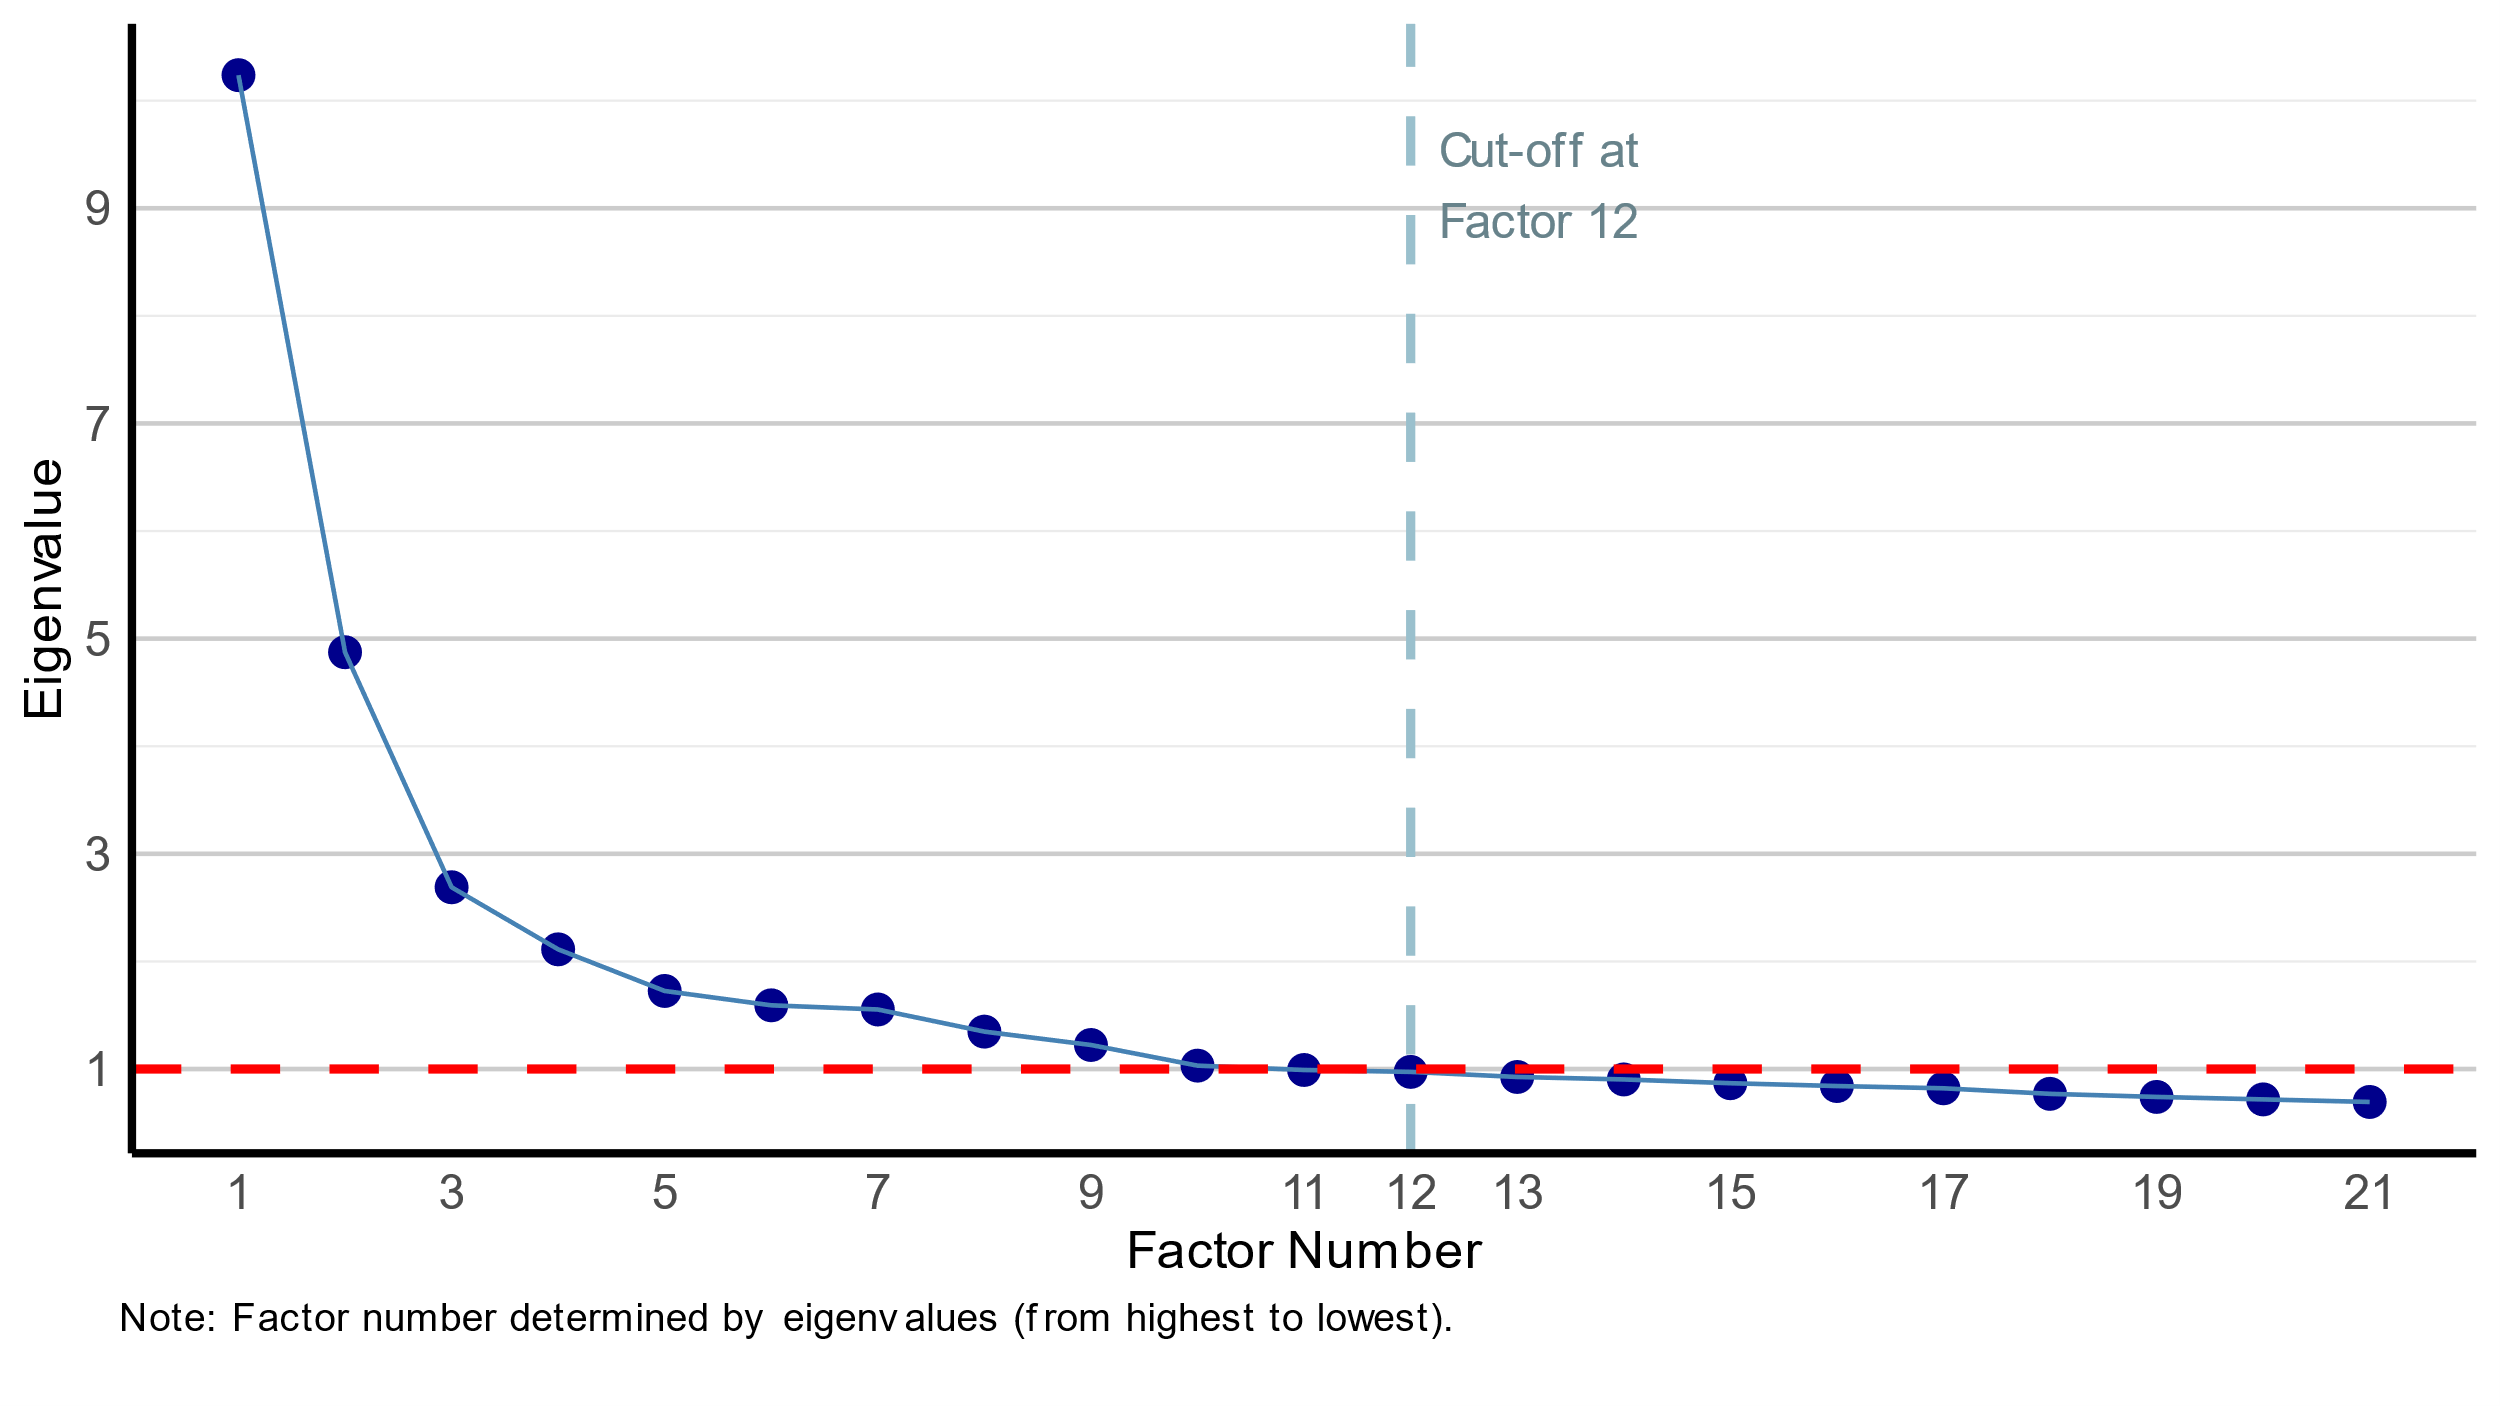
\includegraphics[width=\textwidth]{ai_attitudes_images/image_001.png}
\end{center}

\textbf{Figure A2. Density Plot for Identified Factors (z-standardized).}

\begin{center}
  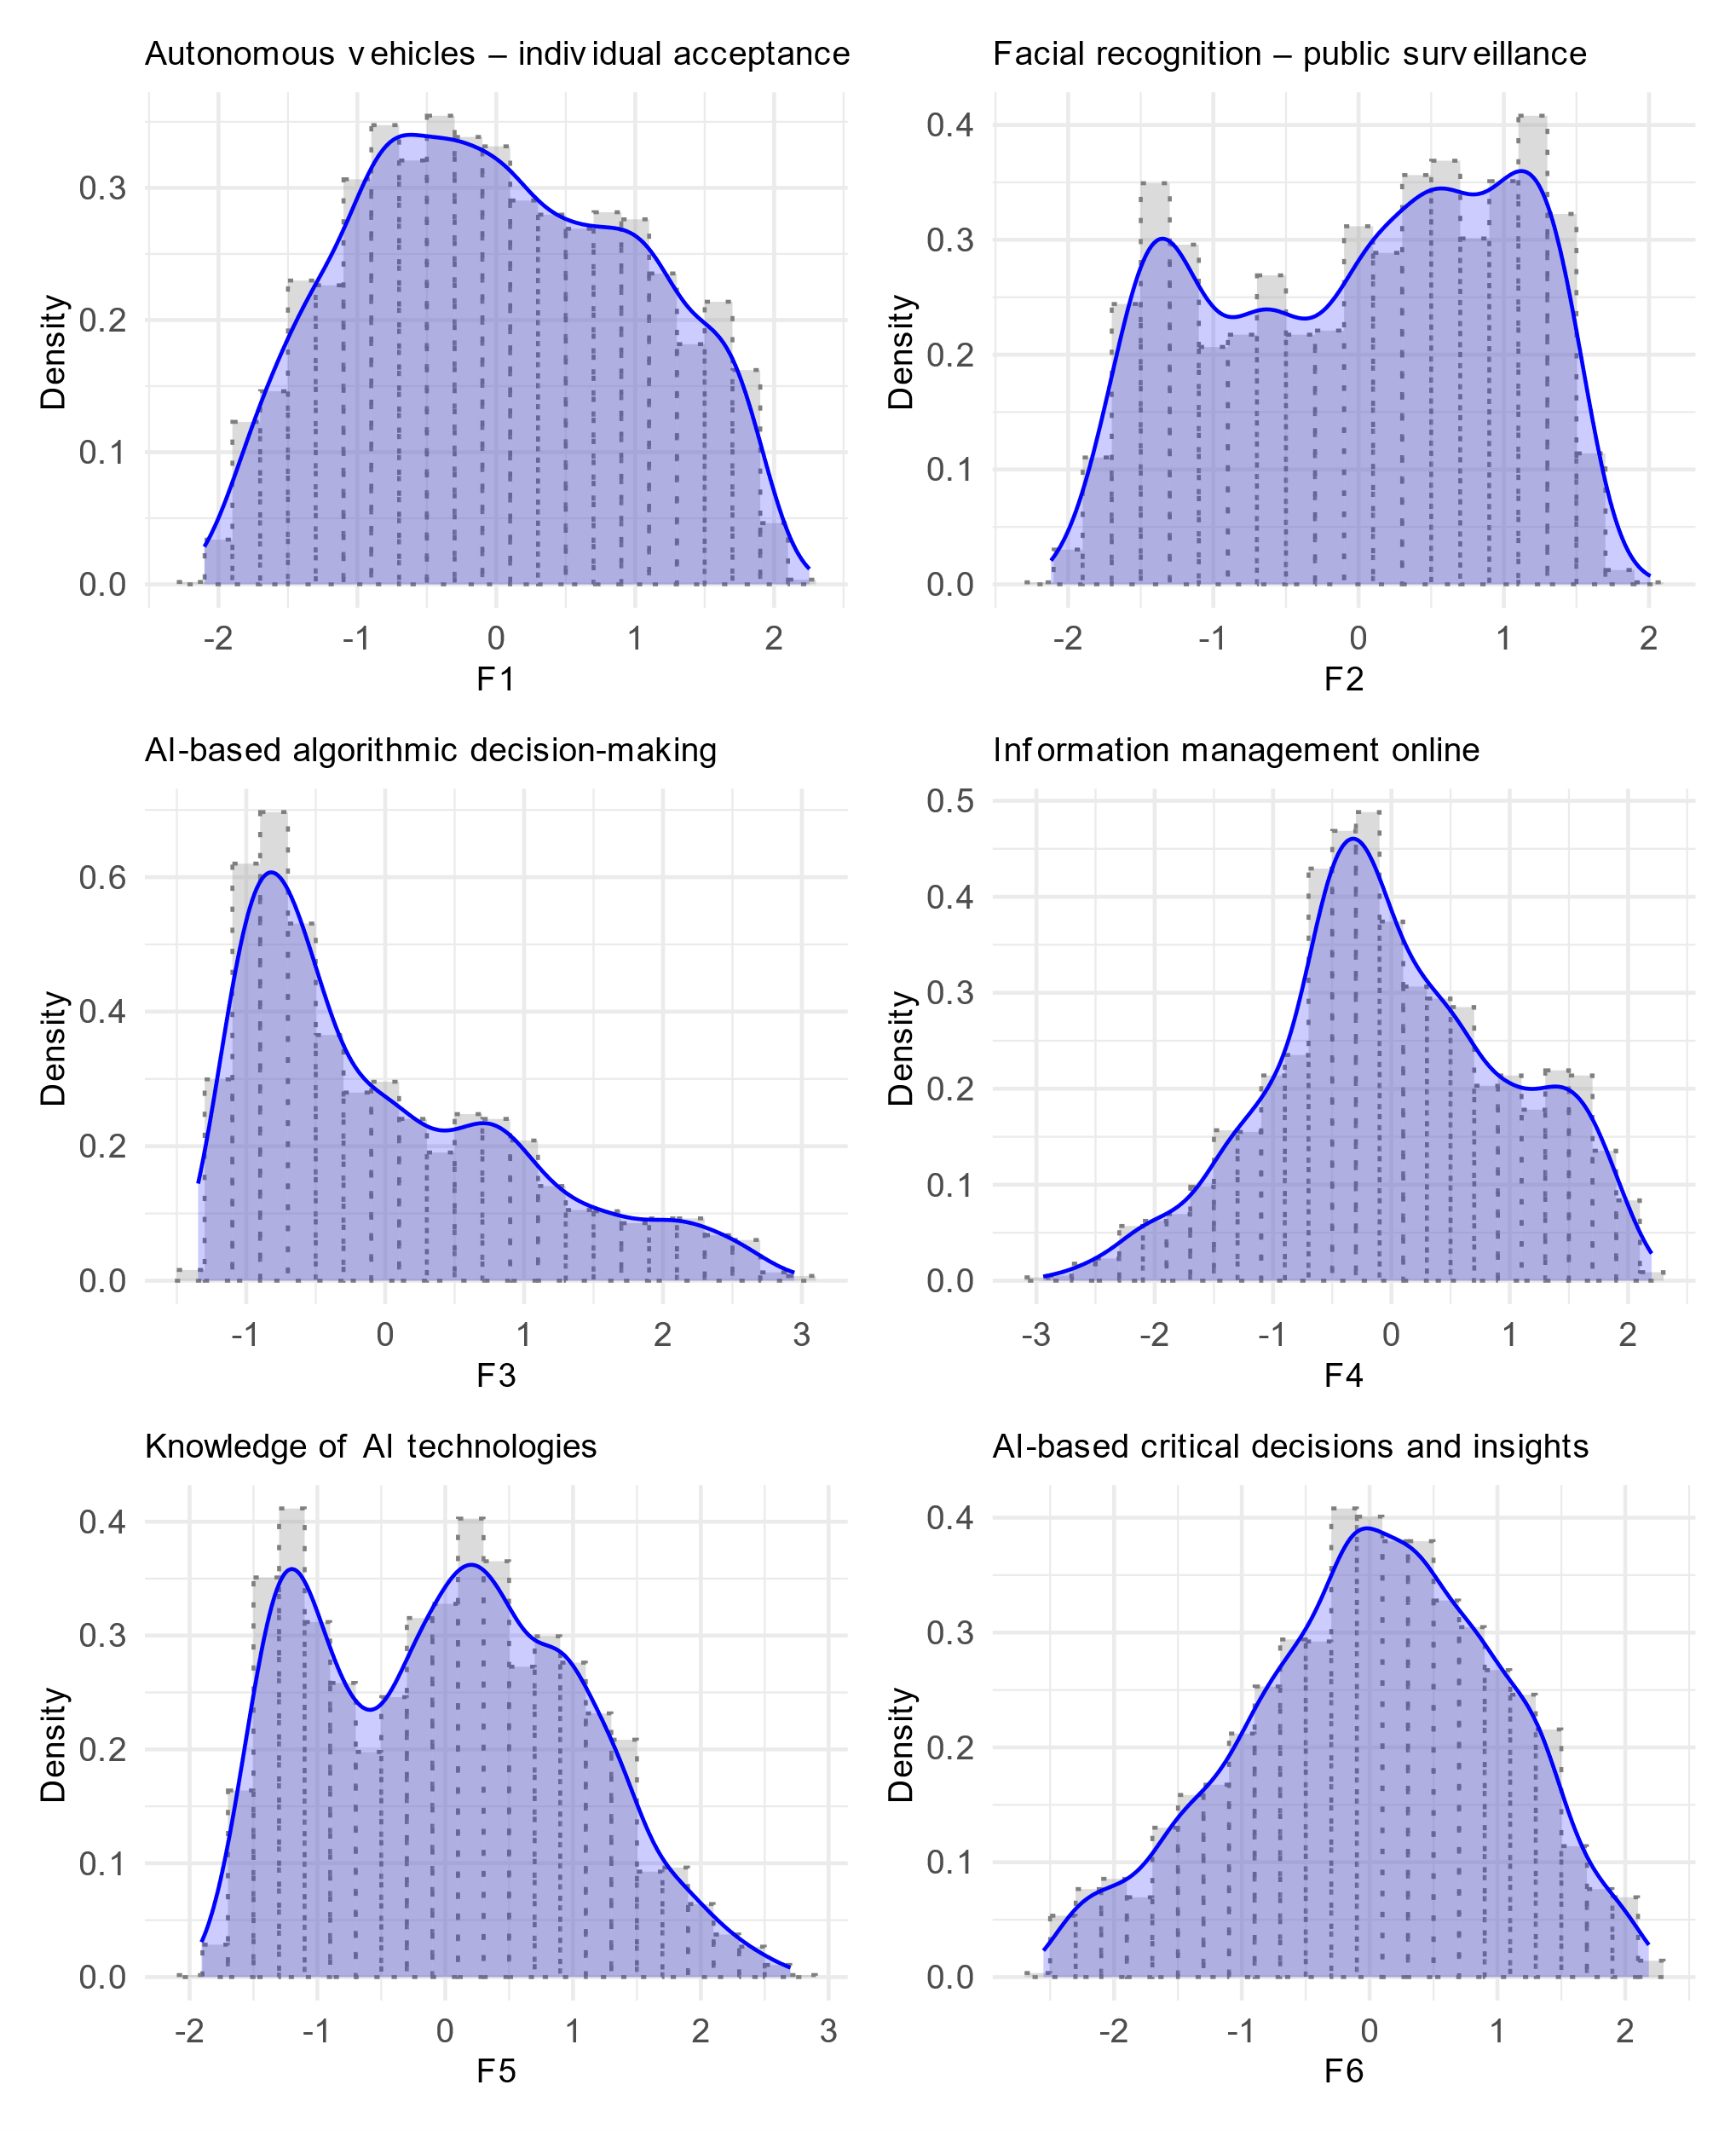
\includegraphics[width=\textwidth]{ai_attitudes_images/image_005.png}
\end{center}

\textbf{Figure A2}\textbf{ (continued)}\textbf{. Density Plot for Identified Factors (z-standardized).}

\begin{center}
  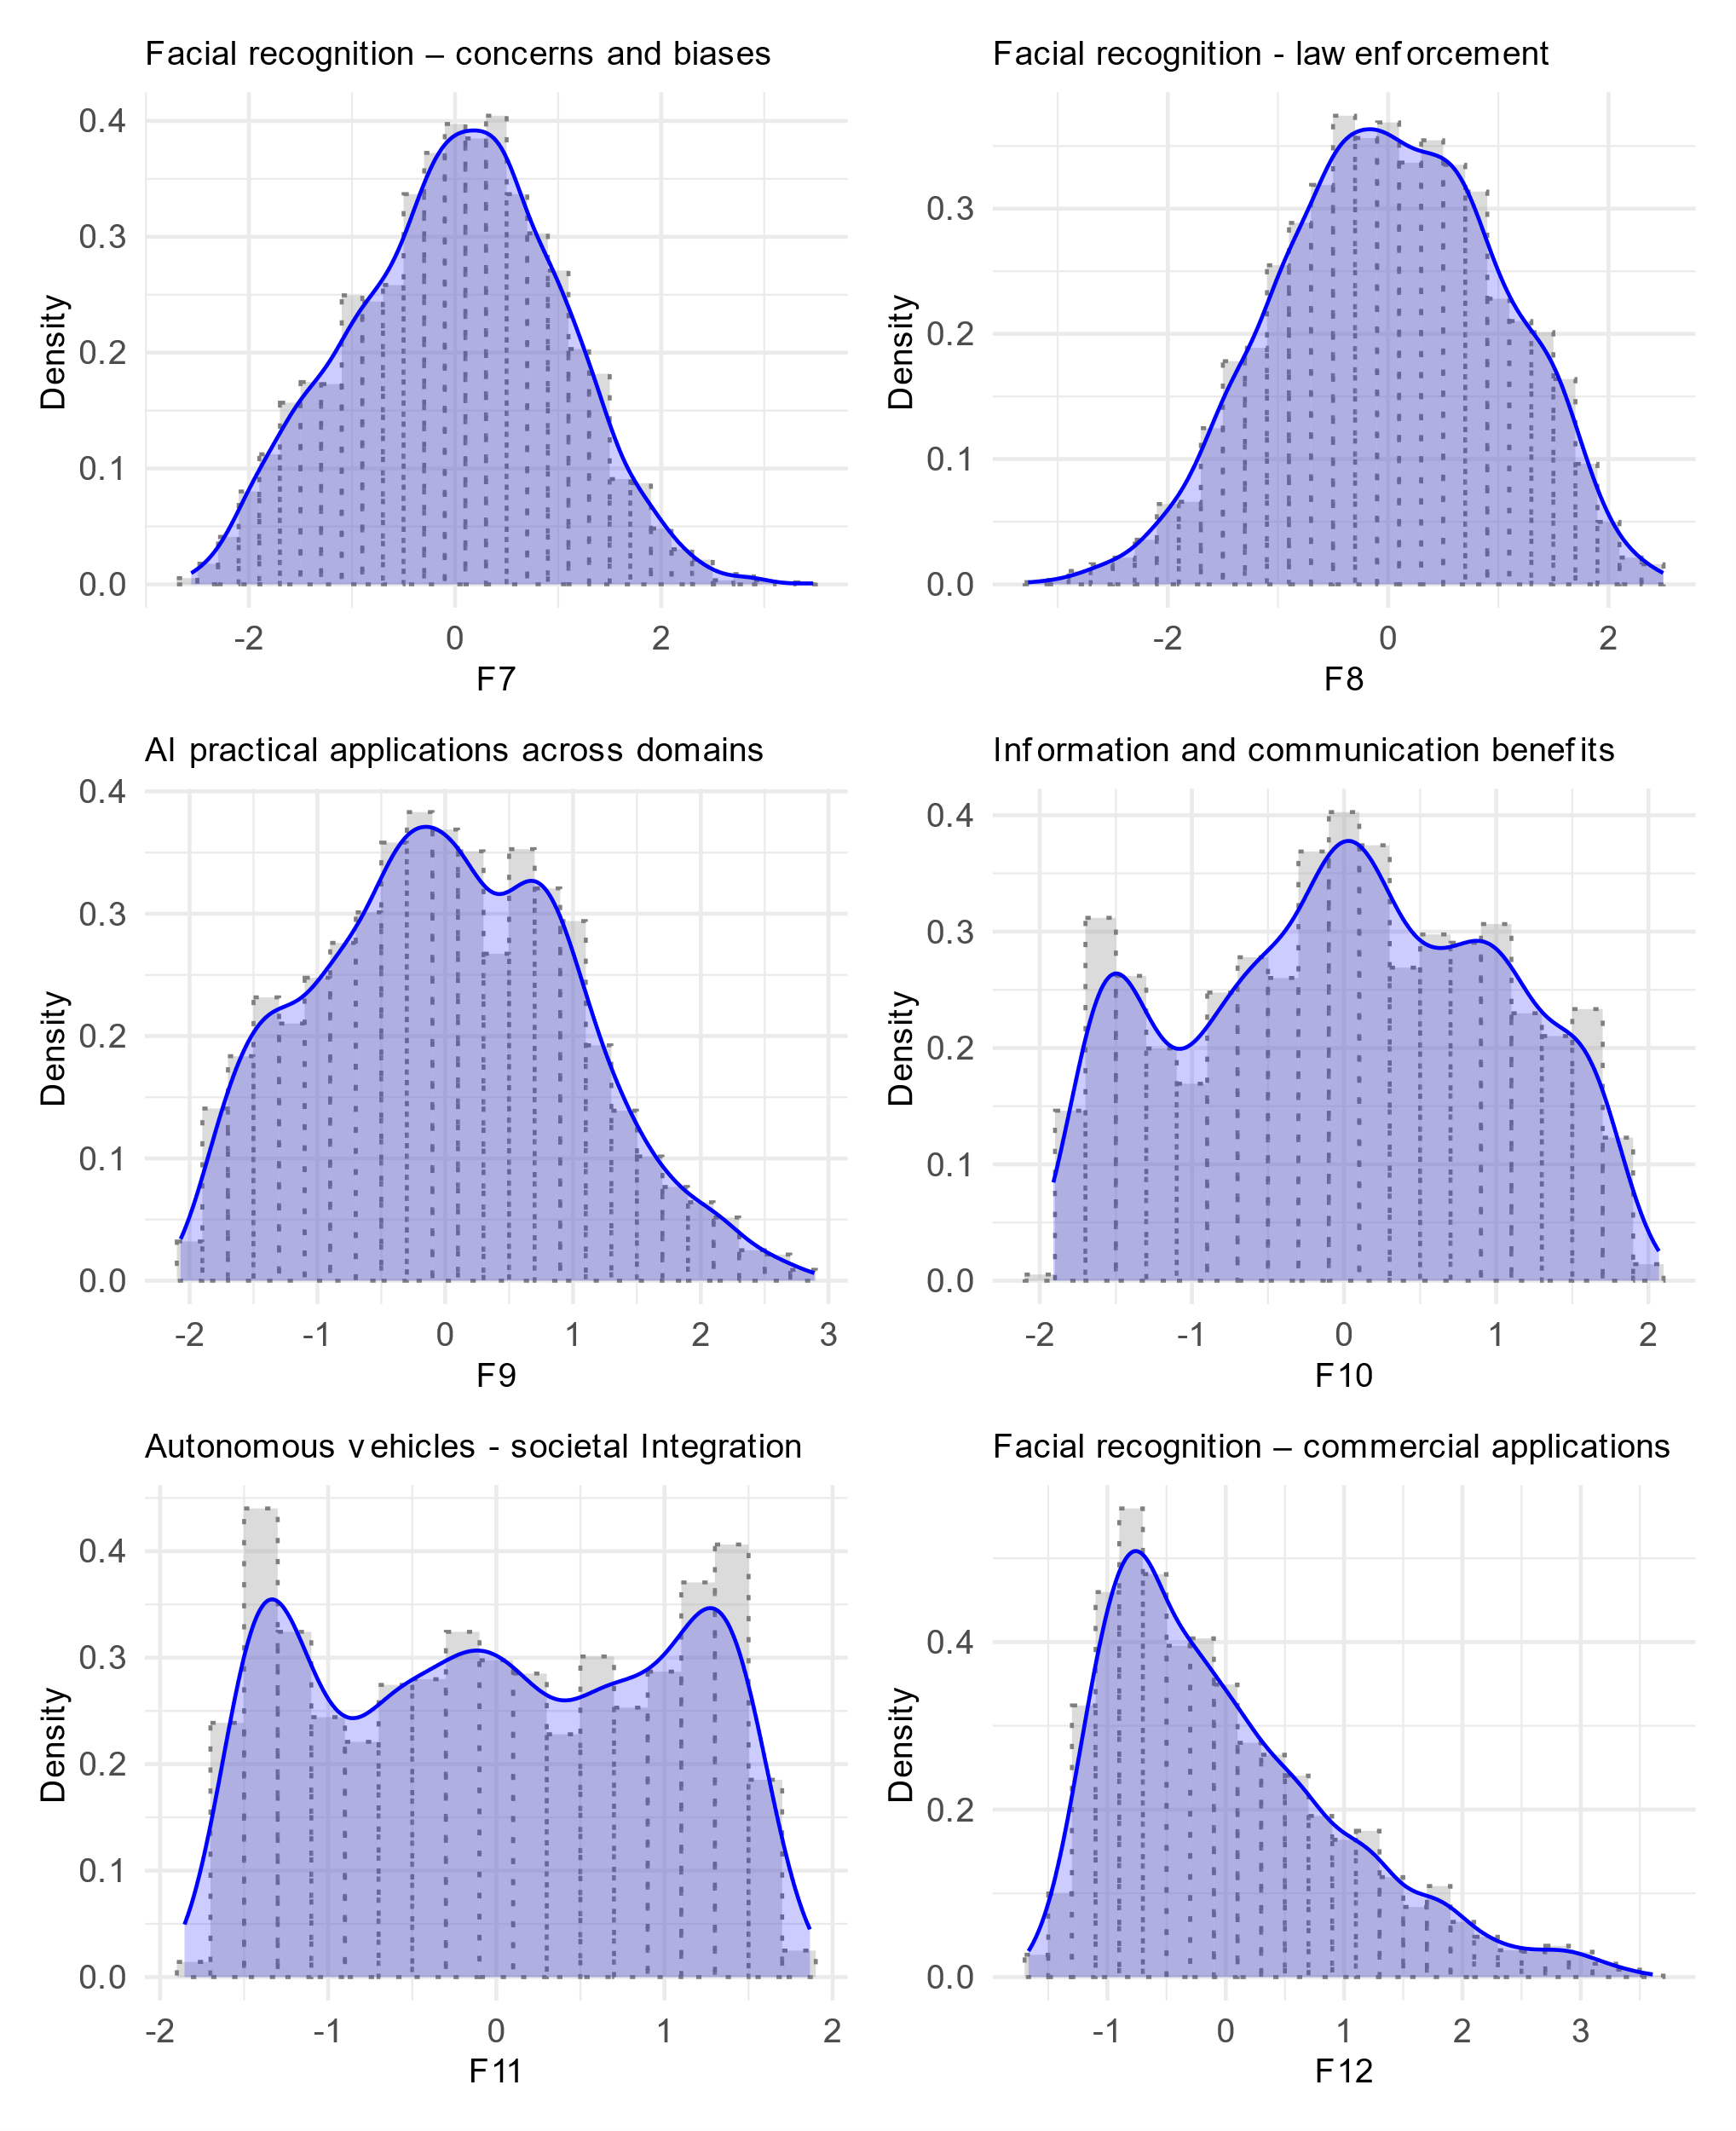
\includegraphics[width=\textwidth]{ai_attitudes_images/image_003.png}
\end{center}

